%!TEX encoding = UTF-8 Unicode
%!TEX TS-program = xelatex
%!BIB TS-program = biber
%%%%%%%%%%%%%%%%%%%%%%%%
\documentclass[12pt,titlepage,oneside]{article}
%%
%% Polices OTF
\usepackage[libertine,libaltvw,liby,vvarbb]{newtxmath}
\usepackage{libertine}
%%%
%% Gestion des langues

\usepackage{polyglossia}
\setdefaultlanguage[frenchfootnote=true,variant=swiss,frenchpart=false]{french}
\setotherlanguage{english}
%% Guillemets
% \RequirePackage[autostyle]{csquotes}
% \MakeOuterQuote{"}
%% Espacement des points-virgules dans les maths
\AtBeginDocument{\mathcode`\;="203B\relax}
%% Format de page
\usepackage{geometry}
\geometry{a4paper}
\geometry{top=25mm, bottom=30mm}
\geometry{outer=20mm, inner=25mm}
\geometry{foot=15mm, head=15pt}
\geometry{footnotesep=5mm}
%% Paragraphes sans indentation, légèrement espacés
\setlength{\parindent}{0pt}
\setlength{\parskip}{5pt plus1pt minus1pt}
\setlength \abovecaptionskip{0.15ex}
%% Interligne
\usepackage{setspace}
\onehalfspacing
%% URLs and hyperlinks
\usepackage[unicode,bookmarks,colorlinks,breaklinks,pdfencoding=auto,psdextra]{hyperref}
\urlstyle{same}
\usepackage{xurl}
\hypersetup{linkcolor=black,citecolor=black,filecolor=black,urlcolor=black}
%% Control table of contents, figures, etc.
\usepackage{tocloft}
%% Flexible tables
\usepackage{tabu}
%% Colors
\usepackage[usenames,dvipsnames,svgnames]{xcolor}
%% Divers outils
\usepackage{xifthen}
\usepackage{array}
\usepackage{tabularx}
\usepackage{multirow}
\usepackage{enumerate}
\usepackage[bottom]{footmisc}

%% Affichage de code
\definecolor{mybackcolor}{rgb}{0.9,0.9,0.9}
\definecolor{mygreen}{rgb}{0,0.5,0}
\usepackage{listings}
\lstdefinestyle{MyFrame}{backgroundcolor=\color{mybackcolor}, basicstyle=\ttfamily\footnotesize, stringstyle=\color{mygreen}, commentstyle=\itshape\color{gray}, numbers=left, frame=single, numbersep=5pt, belowcaptionskip=1\baselineskip, breakatwhitespace=true, showstringspaces=false, breaklines=true, captionpos=b}
\lstdefinestyle{MyHTML} {language=HTML, style=MyFrame}
\renewcommand{\lstlistingname}{Code}

%% Entêtes et pieds de page
\usepackage{fancyhdr}
\pagestyle{fancy}
\fancyhf{} % clear all header and footer fields
\fancyfoot[R]{\thepage}
\renewcommand{\headrulewidth}{1pt}
\renewcommand{\footrulewidth}{0pt}
\fancyhead[R]{\emph{\titlename}}
\fancyfoot[R]{\thepage}
%% Table des matières et numérotation des sections
\setcounter{tocdepth}{3}
\setcounter{secnumdepth}{3}
\gappto\captionsfrench{\renewcommand{\contentsname}{Table des matières}}
%% Illustrations
\usepackage{graphicx}
\graphicspath{{images/}}
\usepackage{float}
%% Commande pour texte en exposant
\let\up\textsuperscript
%% Commande pour supprimer les images, notes de bas de page, etc.
\newif\ifreducedcopy
%% Mettre \reducedcopyfalse pour une copie normale et
%% \reducedcopytrue  pour une copie prête pour détection de plagiat
\newcommand{\authorname}{Caroline Blank}
\newcommand{\tutorname}{Prof. Dr. Jacques Pasquier\\
Software Engineering Group\\}
\newcommand{\titlename}{t-doc}
\newcommand{\subtitlename}{Un écosystème pour la génération de pages Web\\ pour enseignants de mathématiques et informatique}
\newcommand{\worktype}{Travail personnel - Informatique+30}
\newcommand{\workdate}{Mars 2024}
\newcommand{\supervisorslabel}{Supervisé par}
\reducedcopyfalse
\ifreducedcopy
	\setkeys{Gin}{draft}
	\renewcommand{\authorname}{Auteur Anonyme}
	\renewcommand{\tutorname}{Tuteur Anonyme}
	\renewcommand{\footcite}[1]{}
	\renewcommand{\smartcite}[1]{}
	\renewcommand{\footnote}[1]{}
	\renewcommand{\cite}[1]{}
\fi

\newcommand{\titlepagefooter}{
\begin{tabular}{lcr} \hline
\multirow{5}{*}{
\includegraphics[height=1.65cm]{unifr_logo}} &  & \multirow{5}{*}{
\includegraphics[height=1.65cm]{softeng}} \\
& Groupe Génie Logiciel &  \\
& Département d'Informatique &  \\
& Université de Fribourg (Suisse) &  \\
& & \\
\end{tabular}
}

%%
%% Début du document
\begin{document}

\begin{titlepage}
\begin{center}

  \vspace*{0.3cm}
  \begin{huge}
    \textsc\titlename \\
  \end{huge}
  \vspace{0.4cm}
  \begin{Large}
  \subtitlename
  \end{Large}
  \par

  \vspace{0.5cm}
  <\url{https://github.com/t-doc-org/t-doc-v1}>


  %Here you can put your own project logo, if you have one
  %\vspace{1cm}
  %\includegraphics[height=1.5cm]{figures/projectLogo.eps}

  \vspace*{2cm}

  \begin{normalsize}
  \textsc{\worktype}
  \end{normalsize}

  \vspace*{1.5cm}
  \begin{LARGE}
  \textsc{\authorname}\\
      \vspace{0.2cm}
  \end{LARGE}
  \begin{large}
    {\workdate}
  \end{large}

  \vspace*{3cm}

  \textbf{\supervisorslabel}:\\
  \vspace{0.2cm}
  \tutorname
  \vspace*{2cm}

  \titlepagefooter


\end{center}
\end{titlepage}

\section*{Résumé}
Le but du projet est de faciliter la réutilisation de documents existants pour les mettre à disposition des élèves sur le Web. L'enseignant enrichit ses documents en LaTeX par du code Python, des vidéos et des fenêtres Geogebra.

Le coeur du projet est constitué d'un moteur de rendu qui transforme le document rédigé en LaTeX, complété par des balises personnalisées, en une page HTML.  Pour le cours de mathématiques, l'élève pourra visionner dans un navigateur une page qui contient des parties de texte et de contenu mathématique, par exemple, de la théorie, des exercices ou des solutions, une illustration géométrique en utilisant une fenêtre Geogebra, ainsi que des compléments de théorie ou des exemples détaillés en format vidéo. Dans le cadre du cours d'informatique, les pages pourront, en plus, afficher du code surligné afin de faciliter la compréhension et exécuter du code directement dans le navigateur. Cela donne une séquence d'enseignement en autonomie pour la découverte d'une nouvelle notion, la possibilité de revoir une notion pas bien comprise ou tout simplement de réviser pour un examen.

\newpage

\tableofcontents
\thispagestyle{empty}

\clearpage

\setcounter{page}{1}
\section*{Introduction}
\addcontentsline{toc}{section}{Introduction}
T-doc (teaching docs) constitue une mise en pratique des connaissances acquises lors de la formation universitaire en informatique. Le projet a été choisi de manière à répondre à un besoin constaté depuis quelques années et pourra être utilisé dans mon enseignement.\par

En tant qu'enseignante au collège, la préparation des supports de cours prend un temps considérable, notamment la rédaction de document LaTeX. Depuis la rentrée 2022-2023, les élèves des collèges fribourgeois sont passés en mode BYOD \footnote{Bring Your Own Device}, ils ont donc un ordinateur à portée de main à chaque cours. Actuellement, beaucoup d'enseignants se limitent à transmettre leurs cours en format PDF par manque de temps et de motivation à faire mieux. Mais un polycopié en format PDF n'apporte rien de plus aux élèves que sa version papier. Le Web regorge de matériel pédagogique que ce soient des vidéos, des exercices en ligne, des outils pour faire de la géométrie interactive, etc. Malheureusement il est difficile pour les élèves de trouver les bonnes ressources adaptées à leur niveau. C'est ainsi qu'est apparue l'idée de créer un outil qui combine du LaTeX, du Python, des images, des vidéos et des figures Geogebra pour un rendu en une page HTML qui peut être visualisée et avec laquelle on peut interagir dans un navigateur. Les élèves profitent ainsi, en plus du polycopié, d'outils à disposition pour la découverte d'une nouvelle notion, la possibilité de revoir une notion pas bien comprise ou tout simplement de réviser pour un examen.\par

Le coeur du projet est constitué d'un moteur de rendu qui transforme le document d'origine contenant du LaTeX en une page HTML. Pour le cours de mathématiques, l'élève pourra visionner dans un navigateur une page qui contient des parties de texte et de contenu mathématique, par exemple, de la théorie, des exercices ou des solutions, une illustration géométrique en utilisant une fenêtre Geogebra, ainsi que des compléments de théorie ou des exemples détaillés en format vidéo. Dans le cadre du cours d'informatique, les pages pourront, en plus, afficher du code surligné afin de faciliter la compréhension et exécuter ce code directement dans le navigateur. Cela donne des séquences d'enseignement en autonomie.\par

Afin d’illustrer au mieux le projet, le présent rapport est structuré comme suit. Le chapitre 1 présente le cahier des charges. Le chapitre 2 décrit son implémentation sous forme d'une application Web. Le chapitre 3 démontre les fonctionnalités disponibles et comment les utiliser. Le chapitre 4 présente les pistes suivies et rejetées. Le chapitre 5 illustre les difficultés rencontrées tout au long du projet. Et pour terminer, le chapitre 6 décrit les potentielles améliorations futures.\par


\newpage

\section{Cahier des charges}
Cette section définit un cahier des charges des fonctionnalités. Elle précise le profil des utilisateurs cibles. Ensuite, en se mettant à leur place, il faut déterminer les fonctionnalités nécessaires et celles qui sont plutôt optionnelles et qui seront développées plus tard.\par

\subsection{Personas}
Pour ce projet, on considère deux personas: les enseignants et les élèves.\par
Cet outil s'adresse à des enseignants de mathématiques du collège qui ont donc des connaissances en LaTeX et des enseignants d'informatique qui, s'ils ne connaissent pas LaTeX, peuvent facilement acquérir les bases nécessaires.\par
L'enseignant doit pouvoir:
\begin{itemize}
\item adapter rapidement ses documents LaTeX pour la création de pages Web,
\item créer de nouveaux documents,
\item éditer des documents existants,
\item visualiser le rendu des documents de manière itérative.
\end{itemize}
L'enseignant utilisera un éditeur de son choix pour créer les documents.\par
L'élève doit pouvoir:
\begin{itemize}
\item apprendre une nouvelle notion,
\item revoir une notion pas bien comprise en classe,
\item réviser pour un examen.
\end{itemize}
L'élève aura à disposition des séquences d'enseignement en autonomie sous forme de pages Web. Il aura donc besoin d'un navigateur et de l'URL pour accéder à la page.\par

\newpage

\subsection{LaTeX}
LaTeX est un langage qui permet de structurer un document et son contenu. La rédaction des documents se fait sous forme de texte pur avec des balises pour définir la structure, ainsi n'importe quel éditeur peut être utilisé. Ensuite, le code source est traité par un compilateur, par exemple xelatex ou luatex, qui va générer, en général, un document PDF dont la mise en page est effectuée automatiquement. Il est beaucoup utilisé par les enseignants de mathématiques, car il permet un très bon rendu des formules mathématiques. En effet, TeX, le précurseur de LaTeX, a été créé dans les années 70 par Donald Knuth dans ce but.\par

Les enseignants de mathématiques du collège rédigent leurs documents de cours en LaTeX, car il permet d'écrire "facilement" du contenu mathématique. Il est donc essentiel que ce projet intègre LaTeX. Il se focalise, dans un premier temps, sur la compatibilité des commandes standards utilisées pour l'enseignement des mathématiques, c'est-à-dire les formules (environnement mathématique), les symboles, les listes ordonnées ou non-ordonnées (enumerate et itemize), l'affichage avec des colonnes multiples (multicols), les tableaux (array et tabular) et les images. Le support pour des commandes moins utilisées sera ajouté par la suite.\par

\subsection{Multimédia}
Depuis plusieurs années, l'apprentissage au moyen de vidéos est très apprécié, notamment par les adolescents. Cela ne remplace pas un enseignement en classe par un professeur qui est disponible et pourra répondre aux questions, mais cela permet d'apprendre à son rythme, seul et à n'importe quel moment du jour ou de la nuit. Il est souvent plus simple pour les élèves de regarder une vidéo que de lire un polycopié. Pour ces raisons, l'ajout de vidéo était une nécessité. Comme il existe beaucoup de vidéos de qualité d'enseignants de mathématiques sur Youtube, notamment celles d'Yvan Monka \footnote{\url{https://www.youtube.com/@YMONKA}}, le projet n'intégrera, dans un premier temps, que des vidéos Youtube.\par
Toucher et tester facilitent les apprentissages. Pour les mathématiques, Geogebra est un logiciel interactif de géométrie, d'analyse, de statistique et de calcul différentiel. En l'intégrant dans ce projet, les élèves peuvent expérimenter "en live" différentes approches.\par

\newpage

\subsection{Programmation}
Le langage de programmation utilisé dans les collèges fribourgeois est principalement le Python.\par
Lors de l'enseignement de la programmation, il y a plusieurs contraintes à suivre:
\begin{itemize}
\item Les élèves débutent en programmation, il leur est difficile de lire et comprendre du code. Un surlignement de code correct, si possible proche des éditeurs standards, facilite la compréhension par les élèves.
\item L'exécution de code, directement sur la page, permet aux élèves d'essayer de comprendre un programme et ensuite de l'exécuter pour valider ou non leur réponse. Cela leur permet d'avoir un feedback instantané sans que l'enseignant doive valider la réponse.
\item Le module Turtle permet de faire de la programmation visuelle. Le dessin lui-même permet de valider ou non la réussite de l'exercice. Ce module est très souvent utilisé par les enseignants du collège, il est donc nécessaire de pouvoir aussi exécuter du code qui utilise ce module.
\end{itemize}

\newpage

\section{Design et réalisation}
Dans cette partie, les différents outils utilisés et les choix effectués seront présentés et expliqués. Le code source de ce projet est disponible sur GitHub: <\url{https://github.com/t-doc-org/t-doc-v1}>.\par

\subsection{Framework Web}
Comme j'enseigne le Python à mes élèves, je souhaitais l'utiliser pour ce projet et peut-être l'utiliser avec les élèves dans le cadre de l'option complémentaire d'informatique, afin qu'ils développent eux-mêmes une application Web. Parmi les nombreux outils pour développer une application Web, mon choix s'est porté sur Django \cite{django}, un framework Web en Python, parce que je l'ai déjà utilisé dans un autre projet et qu'il a de nombreux avantages, entre-autres:
\begin{itemize}
\item Il est gratuit et open source.
\item Il intègre un serveur Web qui permet de développer et tester une application en temps réel sans déploiement.
\item Il fournit une fonctionnalité de cache flexible.
\end{itemize}

\subsection{Traitement côté client ou côté serveur}
Dans une application Web, le traitement peut, en général, être librement placé du côté du client ou du côté du serveur, voire même être réparti entre les deux. Le client possède un avantage majeur de sécurité, grâce au bac à sable sécurisé du navigateur. Mais de manière générale, il est difficile d'exécuter des logiciels arbitraires dans le navigateur, et une réimplémentation est souvent nécessaire. À l'opposé, le serveur permet de facilement exécuter n'importe quel logiciel, mais une faille dans celui-ci peut compromettre tout le serveur, et donc tous ses utilisateurs. Dans la mesure du possible, ce projet effectuera le traitement du côté client autant que possible, et du côté du serveur si nécessaire.\par

\newpage

\subsection{Format du document d'origine}
L'application doit générer du HTML à partir d'un document pouvant contenir du LaTeX, par conséquent, choisir HTML ou LaTeX comme format du document source semble une évidence. Dans un premier temps, HTML a été privilégié, car il s'agit d'un format plus cohérent et activement développé, mais cette option a été abandonnée par la suite \footnote{voir \nameref{AlternativesConsidérées}}.\par
L'utilisation  de LaTeX comme format d'origine oblige à faire le rendu côté serveur, puisque le navigateur ne comprend pas le LaTeX. Même si cela implique de devoir gérer un serveur, ce choix à l'avantage de faciliter le travail de l'utilisateur. En effet, les enseignants pourront utiliser leurs documents rédigés en LaTeX moyennant quelques modifications, afin d'ajouter les fonctionnalités interactives.\par

\subsection{Génération d'une page HTML à partir d'un document LaTeX}
Il existe différents outils \footnote{voir \nameref{Outils}} qui permettent de convertir du LaTeX en HTML. La qualité du rendu, notamment des formules mathématiques, est très variable. Au niveau de l'utilisation, certains permettent de générer des fragments de LaTeX, mais la plupart requièrent la génération d'un document complet.\par

Lors de mes recherches, deux outils ont particulièrement retenu mon attention:
\begin{enumerate}
\item LaTeX.js \cite{latex.js}, une librairie JavaScript.
\item Make4ht \cite{make4ht}, un package contenu dans la plupart des distributions LaTeX.
\end{enumerate}
Le premier outil a été testé, mais finalement abandonné \footnote{voir \nameref{AlternativesConsidérées}}, car il ne permettait pas le rendu de toutes les fonctionnalités LaTeX souhaitées.\par
Make4ht est un système de construction simplifié pour TeX4ht \cite{tex4ht} lui-même, un convertisseur de TeX en HTML. Make4ht contient un outil en ligne de commande qui gère le processus de conversion configurable. Contrairement à d'autres convertisseurs comme LaTeX2HTML, qui convertissent le document TeX directement en HTML, TeX4ht utilise le fichier DVI \footnote{DeVice-Independent} résultant de la compilation "normale" en entrée. Cela permet une reproduction plus fidèle du document.\par

Pour générer le rendu depuis Django, la commande suivante est exécutée:
\begin{lstlisting}[style=MyHTML, caption = Ligne de commande pour le rendu]
$ make4ht -c latex.cfg -j "output" "monfichier.tex" "mathjax"
\end{lstlisting}
\vspace{-0.5cm}
Cette commande génère deux documents: le fichier HTML (output.html) et le fichier CSS (output.css) qui définit la mise en page. Afin de simplifier le transfert au navigateur, le CSS est ensuite intégré directement dans l'entête du document HTML.\par

\subsection{Affichage de contenu mathématique}
Make4ht permet de configurer le rendu de contenu mathématique. Par défaut, le rendu se fait en MathML, mais la qualité n'est pas acceptable. Il est aussi possible de générer des images SVG. Même si la qualité du rendu est très bonne, ces images ne sont pas stockées directement dans le HTML, mais dans des fichiers séparés. Cela complique le transfert au navigateur, car il faudrait soit garder toutes les références et transmettre plusieurs fichiers, soit inclure les images directement dans le fichier HTML. De plus, les formules sous forme d'image empêchent leur recherche. La solution retenue qui est la plus simple, est d'utiliser MathJax \cite{mathjax}. MathJax est un moteur d'affichage JavaScript open source pour les notations LaTeX, MathML et AsciiMath qui fonctionne dans tous les navigateurs modernes. Il ne nécessite aucune installation.\par

\newpage

\subsection{Ajout de balises personnalisées}
LaTeX permet de créer ses propres macros afin de faciliter la rédaction de documents. Cette possibilité sera utilisée pour la définition de nouvelles balises personnalisées, ainsi l'enseignant pourra intégrer facilement les nouveaux éléments (vidéos, code, solutions, \dots) dans son document LaTeX.\par
Ces balises personnalisées seront traitées lors de la génération du document avec Make4ht à l'aide du fichier de configuration. Celui-ci remplace la balise \textbackslash begin\{document\} du document LaTeX par le contenu du fichier de configuration qui contient, par exemple, des nouvelles commandes ou des nouveaux environnements.\par
Le rendu des balises personnalisées utilise une combinaison de trois techniques:
\begin{itemize}
\item Les transformations se font directement lors du rendu LaTeX:\\
Les balises sont remplacées directement par du code HTML. Ce procédé est utilisé pour les images, les vidéos et les fenêtres Geogebra.
\item Les manipulations se font grâce à du CSS:\\
Ce procédé est utilisé pour l'affichage des solutions. Lors du rendu LaTeX, les balises sont remplacées par des balises <div> avec une classe CSS spécifique. Ainsi le CSS pourra traiter les blocs de solutions correctement.
\item Les manipulations se font côté client en JavaScript:\\
Lors du rendu LaTeX, les balises sont remplacées par des balises HTML <div> avec une classe CSS spécifique. Cela permettra à JavaScript de les retrouver et de surligner le code ou de l'exécuter correctement.
\end{itemize}

\subsubsection{Vidéo}
LaTeX contient des packages pour ajouter des vidéos à un PDF, mais cela ne permet pas d'afficher et de pouvoir visionner des vidéos Youtube sur un site Web à partir de sa référence. Cette transformation se fait directement lors du rendu LaTeX, grâce à une balise personnalisée \textbackslash video\{référence\} qui est remplacée par le code HTML d'intégration de vidéos, en tenant compte de la référence passée en paramètre et de la taille de la vidéo. La taille est optionnelle et par défaut à 50\% de la largeur du texte.\par

\subsubsection{Geogebra}
L'affichage d'une fenêtre Geogebra \cite{geogebra} se fait exactement de la même manière que pour les vidéos. Le document doit être, au préalable, sauvegardé en ligne. Par défaut, la taille de la fenêtre est de 100\% de la largeur du texte.

\subsubsection{Code source}
Le surlignement de blocs facilite la lecture et la compréhension. En LaTeX, le package lstlisting permet de le faire facilement, car les principaux langages sont prédéfinis. Toutefois, lors de la génération du document HTML, Make4ht ajoute des balises pour gérer l'indentation. Cela a pour conséquence que ce n'est plus un bloc de code et donc qu'il est impossible de le réutiliser, par exemple pour l'exécuter et afficher le résultat. La solution à ce problème est d'utiliser le package verbatim qui affiche exactement ce qui est écrit, c'est-à-dire qu'il garde l'indentation et les retours à la ligne, mais surtout il conserve le code dans une seule et même balise, ce qui permet de le réutiliser.\par
Le problème de l'indentation étant réglé, il faut maintenant surligner le code. Pour cela, il existe différents outils utilisant du JavaScript. Highlight.js \cite{highlightjs} a été choisi pour sa simplicité d'utilisation. Il permet d'afficher 192 langages avec différents thèmes et fonctionne avec n'importe quel balisage HTML. Il a une fonctionnalité de détection automatique du langage, mais celle-ci ne fonctionne pas toujours correctement, particulièrement lorsque les blocs de code sont courts, comme c'est le cas, dans les exercices que je propose. Par conséquent, l'utilisateur devra toujours indiquer le langage utilisé dans le document LaTeX.\par
Pour utiliser highlight.js, il faut que le code se trouve dans un conteneur HTML <div class="tdoc-code tdoc-lang-NomDuLangage">.\par

\subsubsection{Exécution de code}
Afin de s'assurer que l'élève a compris le code donné, il doit pouvoir l'exécuter dans le navigateur. Skulpt \cite{skulpt}, un outil qui compile du Python en utilisant Javascript, offre une solution simple. En réalité, Skulpt traduit le code écrit en Python en code JavaScript, cela s'effectue côté client, donc directement dans le navigateur. \par
Il y a deux types d'exécution:
\begin{itemize}
\item le résultat est affiché sur la console,
\item le code qui utilise le module Turtle affiche un dessin dans un canevas graphique.
\end{itemize}
Skulpt permet de gérer les deux types d'exécution. L'enseignant détermine si le code pourra être exécuté grâce aux paramètres "interactive" ou "interactive\_turtle", s'il utilise le module Turtle.\par

\newpage
\subsubsection{Solution}
Pour permettre aux élèves de travailler en autonomie, il est nécessaire d'y inclure les solutions. L'idée est d'intégrer ces solutions au document LaTeX et l'élève pourra les afficher sur demande. Les solutions sont placées dans des balises HTML <div class='tdoc-solution'>, ainsi elles pourront être manipulées par la suite par le navigateur.\par

L'affichage ou non des solutions se fait au moyen de CSS. Le principe pour l'affichage des solutions est le suivant: chaque solution a une checkbox invisible associée, si celle-ci est cochée, la solution sera affichée. Par défaut, les solutions ne sont pas affichées.\par

\subsection{Sécurité}
La compilation de documents LaTeX sur le serveur présente des problèmes de sécurité non négligeables. Le compilateur date d'une époque où la sécurité n'était pas primordiale, et il n'a pas été conçu pour traiter des documents de sources non-fiables. Par exemple, il est facile d'écrire un document qui expose des fichiers arbitraires du serveur, ou qui modifie des fichiers existants. Pire encore, bon nombre de failles ont été découvertes qui permettent l'exécution de code arbitraire à travers un document TeX \cite{cve2016} \cite{cve2018}. Il est même possible d'écrire un virus en TeX \cite{usenix}.\par

Ces problèmes peuvent être atténués par des technologies comme l'isolation des processus correspondants dans des conteneurs. Pour des raisons de simplicité et de contraintes de temps, ce projet considère que les documents LaTeX proviennent d'une source fiable, et chaque enseignant aura donc un déploiement séparé pour ses propres documents. Un déploiement partagé sera réalisé plus tard.

\newpage

\subsection{Cache}
La génération de code HTML avec Make4ht, même de documents simples, prend plus de 10 secondes. En effet, Make4ht effectue le rendu trois fois, car certaines informations dépendent du rendu final, comme la table des matières d'un document, le nombre de pages total ou les références croisées. Malheureusement une latence de plusieurs secondes n'est pas acceptable pour les utilisateurs d'un site Web. Deux solutions sont implémentées pour y remédier:
\begin{itemize}
\item L'enseignant peut utiliser une version "draft" lors de la génération du code HTML, ainsi Make4ht exécute le fichier une seule fois. Cela permet de réduire le temps de chargement à environ 4 secondes. Mais cette fonction, pratique lors de la création ou l'édition de documents, ne peut pas être utilisée dans la version finale.
\item L'utilisation d'un cache persistant permet de diminuer de manière significative le temps de chargement de la page. Les pages créées pour ce projet étant statiques, il suffit de les générer à la première utilisation et ensuite de les sauvegarder sur le serveur. Si la page est modifiée, elle sera à nouveau générée.
\end{itemize}
Django intègre un système de cache sur système de fichiers qui stocke les fichiers dans le répertoire "cache", ainsi même si le serveur est arrêté, les fichiers seront préservés. Chaque document sera associé à une clé unique qui détermine sa version. La clé dépend des paramètres suivants:
\begin{enumerate}
\item Un "seed" utilisé pour l'invalidation du cache. Le "seed", défini dans le fichier settings.py du projet Django, permet l'effacement de tout le cache lors de changements qui concernent tous les documents, par exemple une mise à jour de LaTeX.
\item Le contenu du fichier LaTeX.
\item Le contenu du fichier de configuration.
\item Le mode: normal ou draft.
\end{enumerate}
Lors du chargement de la page, le programme détermine la clé en fonction des différents éléments ci-dessus. Ensuite, il vérifie dans le cache si cette version de la page existe déjà. Si c'est le cas, il l'envoie directement au navigateur, sinon il génère la nouvelle page, la stocke et la transmet au navigateur.\par
Ainsi l'affichage d'une page pour un élève ne prend que quelques millisecondes.\par

\newpage

\section{Démonstration d'utilisation - Mode d'emploi}
L'enseignant qui souhaite utiliser cette application, doit pouvoir créer des documents LaTeX avec une structure correcte. Pour cela, il a besoin:
\begin{itemize}
\item de connaissances de base de LaTeX,
\item d'un éditeur de texte,
\item de connaître les balises personnalisées qui peuvent être ajoutées,
\item d'installer le serveur Web qui s'occupera de la génération et du stockage des documents.
\end{itemize}

\subsection{Serveur Web}
Pour créer le serveur Web dans un conteneur Docker \cite{docker}, il faut:
\begin{enumerate}
  \item Installer docker: \url{https://docs.docker.com/desktop/}
  \item Cloner le projet: \url{https://github.com/t-doc-org/t-doc-v1.git}
  \item Se déplacer dans le répertoire t-doc-v1/server.
  \item Créer une image à partir du Dockerfile. Celle-ci contiendra les packages nécessaires (Python3, Django, Texlive).\\
  \$ \texttt{docker build -t t-doc .}
  \item Créer un conteneur basé sur l'image ci-dessus (remplacer REPO par le chemin d'accès du projet cloné ci-dessus).\\
  \$ \texttt{docker create --name=t-doc --publish=8000:8000 \textbackslash\\
  --mount=type=bind,source=REPO,target=/repo,readonly t-doc}\\
  Le code de l'application Web et les documents sont exposés au conteneur en lecture seule. Cela permet d'ajouter et d'éditer les documents normalement, à l'extérieur du conteneur.
  \item Démarrer le conteneur.\\
  \$ \texttt{docker start t-doc}
  \item Pour accéder aux documents, utiliser l'adresse suivante (remplacer DOCUMENT par le chemin d'accès du document, relatif au répertoire Documents, sans l'extension ".tex"):\\
  http://localhost:8000/doc/DOCUMENT
\end{enumerate}

\newpage
Le conteneur ci-dessus est configuré en mode "développement". Pour une mise en production, les pas suivants doivent être effectués:
\begin{enumerate}
  \item Créer un fichier de configuration settings.py dans le répertoire du projet, pour un environnement de production. Entre-autres, les variables Django DEBUG, ALLOWED\_HOSTS et SECRET\_KEY doivent y être surchargées.
  \item Ajouter l'option suivante lors de la création du conteneur:\\
  \texttt{--env=DJANGO\_SETTINGS\_PATH=/repo/settings.py}
\end{enumerate}

\subsection{Édition et création de documents}
\begin{itemize}
\item Tous les documents se trouvent dans le répertoire t-doc-v1/Documents. Ce répertoire peut être hiérarchisé. Cette hiérarchie sera utilisée pour l'affichage des documents dans le navigateur.\\
Exemple: le document Trigonométrie.tex qui se trouve dans le répertoire Géométrie sera appelé avec l'URL suivante:\\
http://localhost:8000/doc/Géométrie/Trigonométrie\par

\item Les images doivent être impérativement sauvegardées, dans le même répertoire, dans un dossier "images".\par

\item Le fichier Template.tex, disponible dans le répertoire Documents, fournit un point de départ pour la création de nouveaux documents.\par

\item L'utilisation des différentes balises personnalisées est expliquée dans le document Tutoriel.tex accessible à l'adresse suivante:\\
\url{http://t-doc.org/doc/Tutoriel}\par

\item S'il y a des erreurs dans le document, les erreurs de Make4ht sont affichées à la place de la page Web.
\begin{figure}[H]
\centering
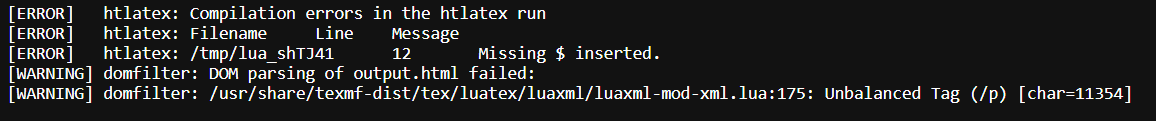
\includegraphics[width=1\textwidth]{images/Erreur.png}\caption{Exemple de message d'erreur affiché dans le navigateur}
\end{figure}
\end{itemize}

\newpage

\subsection{Structure du document LaTeX}
La structure du document LaTeX ne diffère pas beaucoup de la structure standard. Pour simplifier la rédaction et surtout alléger l'écriture de l'entête du document, la liste des packages usuels de LaTeX se trouve dans le fichier commonpackages.sty.
\begin{lstlisting}[style=MyHTML, caption = Fichier commonpackages.sty]
\ProvidesPackage{commonpackages}

\usepackage[french]{babel}
\usepackage[T1]{fontenc}
\usepackage{amssymb,amsmath,amsfonts, amsfonts}
\usepackage{enumitem}
\usepackage{multicol}
\usepackage{graphicx}
\usepackage{media9}
\usepackage{verbatim}
\usepackage{hyperref}
\usepackage{xcolor}

\endinput
\end{lstlisting}
\vspace{-0.5cm}
Voici la structure de base du document avec l'import du package commonpackage et la définition et la création du titre de la page.\par
\begin{lstlisting}[style=MyHTML, caption = Structure de base du document LaTeX]
\documentclass[a4paper,11pt]{article}
\usepackage{commonpackages}

\begin{document}
\title{Noter le titre ici}
\date{}
\maketitle
...
\end{document}
\end{lstlisting}
\vspace{-0.5cm}
Il est nécessaire de définir le titre et d'appeler la commande \textbackslash maketitle, car celle-ci permet de définir le titre du document et le nom de l'onglet de la page HTML.

\newpage

\subsection{Balises personnalisées}
La version Web de cette section se trouve à la page suivante: \url{http://t-doc.org/doc/Tutoriel}.\par
Afin de pouvoir ajouter des vidéos Youtube, une fenêtre Geogebra, des images, du code et des solutions, des balises personnalisées peuvent être ajoutées au document LaTeX. Leur fonctionnement sera expliqué en détail au moyen d'exemples.

\subsubsection{Vidéos Youtube}
Pour ajouter une vidéo Youtube, il suffit de connaître sa référence et d'utiliser la balise suivante: \textbackslash video\{référence\}
\begin{lstlisting}[style=MyHTML, caption = Code LaTeX avec ajout d'une vidéo Youtube]
\documentclass[a4paper,11pt]{article}
\usepackage{commonpackages}

\begin{document}
\title{Produits remarquables}
\date{}
\maketitle
Cette vidéo explique comment développer des produits de polynômes en utilisant les produits remarquables.\par
\video{U98Tk89SJ5M}
\end{document}
\end{lstlisting}
\vspace{-0.5cm}
\begin{figure}[H]
\centering
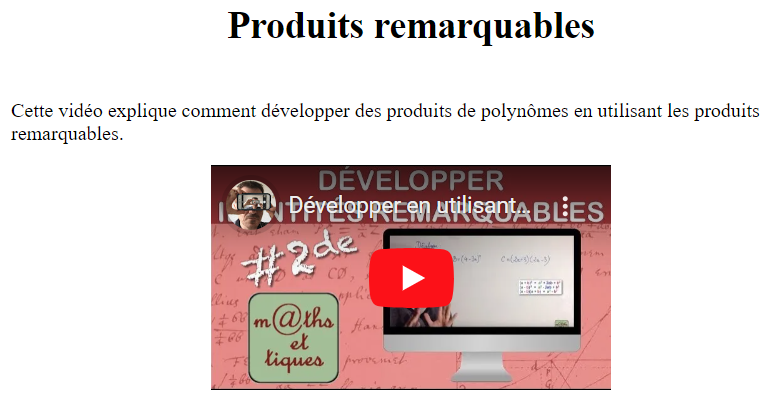
\includegraphics[width=0.9\textwidth]{images/ExempleVideo.png}\caption{Rendu de la page HTML avec une vidéo}
\end{figure}

\newpage

Par défaut, la taille de la fenêtre de la vidéo est 50\% de la largeur du texte. Il est possible de changer la dimension en ajoutant un paramètre optionnel, celui-ci doit être noté entre crochets et avant la référence de la vidéo:
\begin{lstlisting}[style=MyHTML, caption = Code LaTeX pour une vidéo avec une dimension de 100\%]
\video[100]{U98Tk89SJ5M}
\end{lstlisting}
\vspace{-0.5cm}
Les vidéos peuvent être visionnées en plein écran.

\subsubsection{Fenêtres Geogebra}
Pour ajouter une fenêtre Geogebra, il faut tout d'abord créer le document Geogebra et le sauvegarder en ligne <\url{https://www.geogebra.org/}>. Ensuite, il pourra être intégré au document LaTeX au moyen de la balise suivante: \textbackslash geogebra\{référence\}. La structure est la même que pour les vidéos Youtube.
\begin{lstlisting}[style=MyHTML, caption = Code LaTeX avec ajout d'une fenêtre Geogebra]
\documentclass[a4paper,11pt]{article}
\usepackage{commonpackages}

\begin{document}
\title{Équation d'une droite}
\date{}
\maketitle
La fenêtre Geogebra permet à l'élève d'observer comment change la droite en fonction de a qui représente la pente et b qui est l'ordonnée à l'origine:\par
\geogebra{esdhdhzd}
\end{document}
\end{lstlisting}
\vspace{-0.5cm}
\begin{figure}[H]
\centering
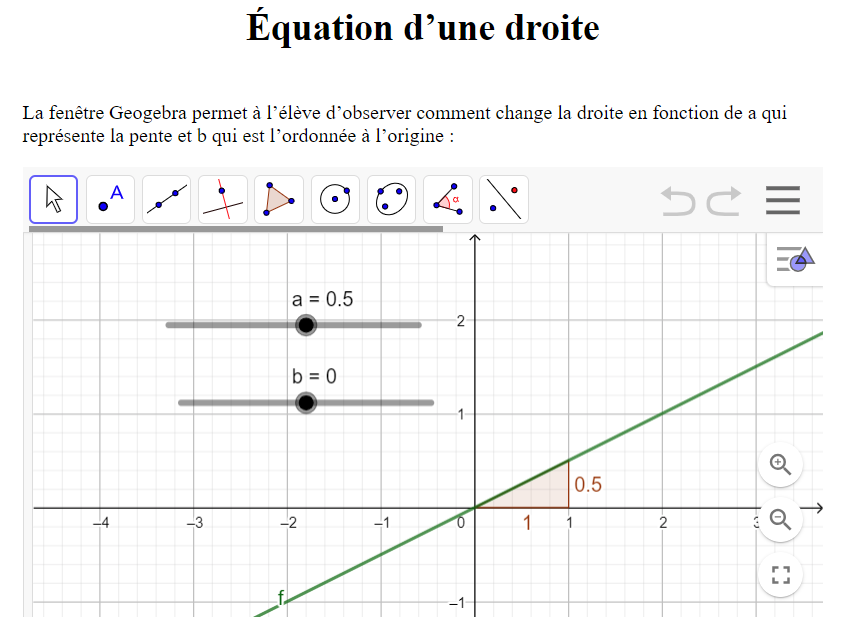
\includegraphics[width=0.9\textwidth]{images/ExempleGeogebra.png}\caption{Rendu de la page HTML avec une fenêtre Geogebra}
\end{figure}
Par défaut, la taille de la fenêtre Geogebra est 100\% de la largeur du texte, afin d'optimiser l'utilisation pour l'élève. Il est possible de changer la dimension en ajoutant un paramètre optionnel, celui-ci doit être noté entre crochets et avant la référence du document Geogebra:
\begin{lstlisting}[style=MyHTML, caption = Code LaTeX pour une fenêtre Geogebra avec une dimension de 75\%]
\geogebra[75]{esdhdhzd}
\end{lstlisting}
\vspace{-0.5cm}
Geogebra peut être utilisé en plein écran.

\subsubsection{Images}
L'ajout d'images ne nécessite pas la création d'une balise personnalisée, toutefois pour que l'affichage soit correct au moment du rendu, il est nécessaire de définir les dimensions de celle-ci en fonction de la largeur du texte (\textbackslash textwidth):
\begin{lstlisting}[style=MyHTML, caption = Code LaTeX avec une image dont la largeur sera 80\% de la largeur du texte]
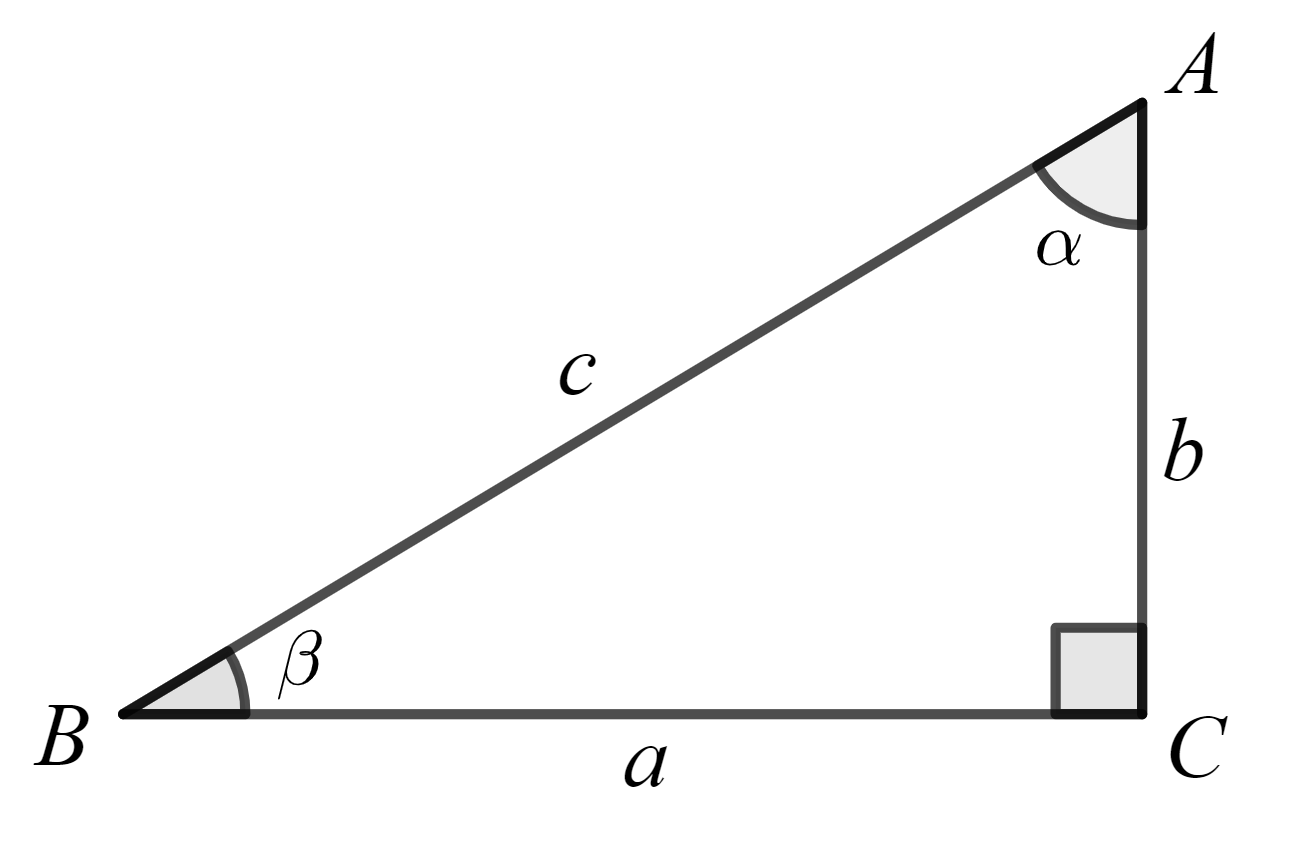
\includegraphics[width=0.8\textwidth]{images/trianglerect.png}
\end{lstlisting}

\newpage

\subsubsection{Code source}
Pour afficher du code source, celui-ci sera simplement inclus dans un environnement code, c'est-à-dire qu'il sera délimité par les balises \textbackslash begin\{code\} et \textbackslash end\{code\}. Afin que le surlignement se fasse correctement, il est obligatoire de définir le langage comme paramètre.
\begin{lstlisting}[style=MyHTML, caption = Code LaTeX avec ajout de code source Python]
\documentclass[a4paper,11pt]{article}
\usepackage{commonpackages}

\begin{document}
\title{Exemple de code en Python}
\date{}
\maketitle
\begin{code}{python}
for i in range(4):
    print(i)
\end{code}
\end{document}
\end{lstlisting}
\vspace{-0.5cm}
Le code est affiché avec une numérotation des lignes et surligné grâce à highlight.js.
\begin{figure}[H]
\centering
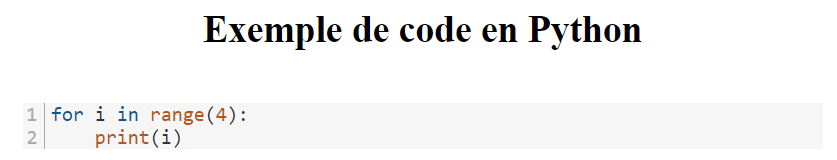
\includegraphics[width=0.9\textwidth]{images/ExempleCodeSource.png}\caption{Rendu de la page HTML avec du code source}
\end{figure}

\newpage
Actuellement, seul le langage Python peut être exécuté dans le navigateur. Pour cela, il faut ajouter le paramètre optionnel "interactive".
\begin{lstlisting}[style=MyHTML, caption = Code LaTeX avec ajout de code source Python exécutable]
\documentclass[a4paper,11pt]{article}
\usepackage{commonpackages}

\begin{document}
\title{Exemple de code en Python}
\date{}
\maketitle
\begin{code}[interactive]{python}
for i in range(4):
    print(i)
\end{code}
\end{document}
\end{lstlisting}
\vspace{-0.5cm}
\begin{figure}[H]
\centering
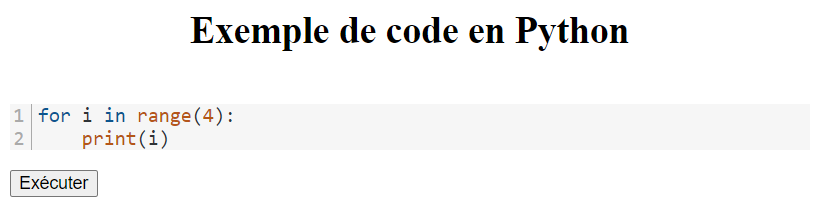
\includegraphics[width=0.9\textwidth]{images/ExempleCodeSourceExecute1.png}\caption{Rendu de la page HTML du code qui pourra être exécuté}
\end{figure}

\begin{figure}[H]
\centering
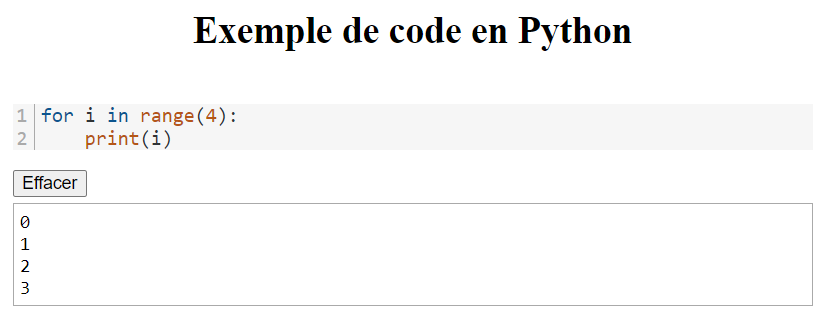
\includegraphics[width=0.9\textwidth]{images/ExempleCodeSourceExecute2.png}\caption{Rendu de la page HTML du code après exécution}
\end{figure}

\newpage

L'affichage de code contenant le module Turtle est fait dans un canevas graphique, il est donc nécessaire de spécifier, quand il est utilisé. Cela se fait au moyen du paramètre optionnel "interactive\_turtle".
\begin{lstlisting}[style=MyHTML, caption = Code LaTeX avec ajout de code source Python exécutable avec le module Turtle]
\documentclass[a4paper,11pt]{article}
\usepackage{commonpackages}

\begin{document}
\title{Exemple de code en Python avec le module Turtle}
\date{}
\maketitle
\begin{code}[interactive_turtle]{python}
from turtle import *
from random import randint

penup()
goto(-100, -100)
pendown()
nb_cote_max = int(input("Combien de côtés voulez-vous au maximum? "))
colormode(255)
pensize(3)
for i in range(3, nb_cote_max + 1):
    for j in range(i):
        forward(100)
        left(360/i)
    pencolor(randint(0,255), randint(0, 255), randint(0,255))
\end{code}
\end{document}
\end{lstlisting}
\vspace{-0.5cm}

\begin{figure}[H]
\centering
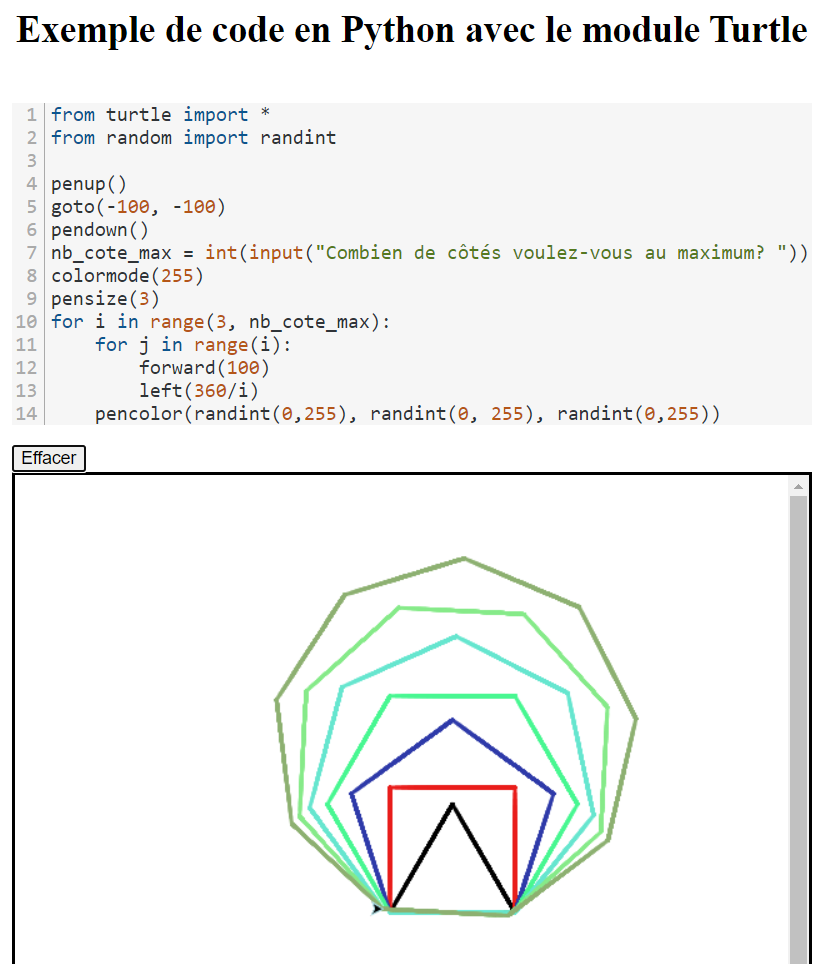
\includegraphics[width=0.9\textwidth]{images/ExempleTurtle2.png}\caption{Rendu de la page HTML du code contenant le module Turtle après exécution}
\end{figure}

\newpage

\subsubsection{Solution}
Afin de pouvoir afficher ou non la solution des exercices, celle-ci sera incluse dans un environnement solution, c'est-à-dire qu'elle sera délimitée par les balises \textbackslash begin\{solution\} et \textbackslash end\{solution\}.
\begin{lstlisting}[style=MyHTML, caption = Code LaTeX avec ajout de solution à un exercice]
\documentclass[a4paper,11pt]{article}
\usepackage{commonpackages}

\begin{document}
\title{Produits remarquables - Exercice}
\date{}
\maketitle

Calculer à l'aide des produits remarquables.
\begin{multicols}{2}
\begin{enumerate}
\item $(x-y)^2=$
\item $(x-1)^2=$
\item $(2c+1)(2c-1)=$
\item $(x-2)(x+2)=$
\end{enumerate}
\end{multicols}

\begin{solution}
\begin{enumerate}
\item $x^2-2xy+y^2$
\item $x^2-2x+1$
\item $4c^2-1$
\item $x^2-4$
\end{enumerate}
\end{solution}
\end{document}
\end{lstlisting}
\vspace{-0.5cm}

\begin{figure}[H]
\centering
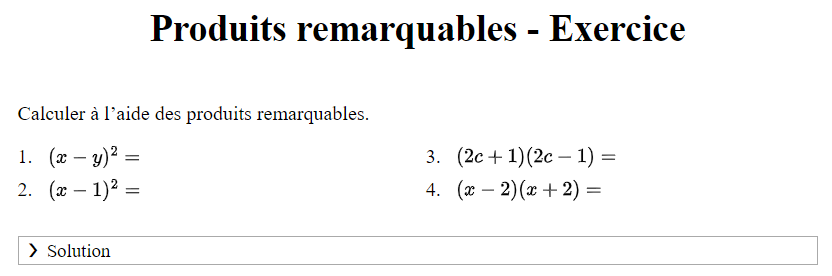
\includegraphics[width=0.9\textwidth]{images/ExempleSolution1.png}\caption{Rendu de la page HTML avec solution cachée}
\end{figure}
\begin{figure}[H]
\centering
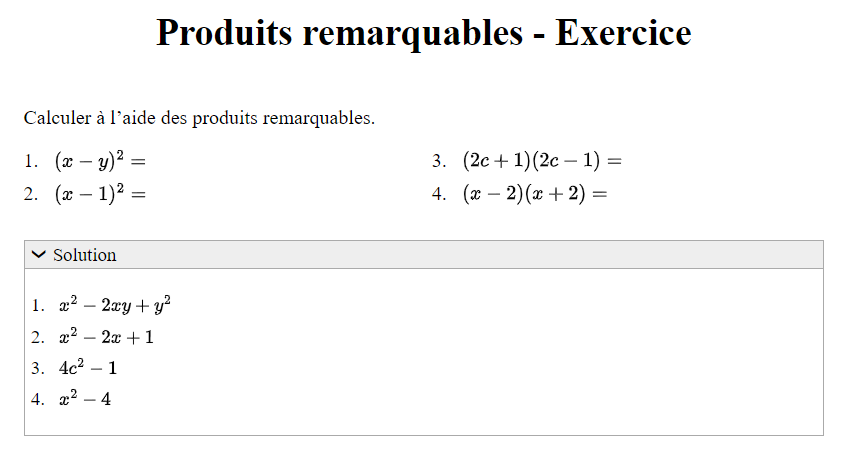
\includegraphics[width=0.9\textwidth]{images/ExempleSolution2.png}\caption{Rendu de la page HTML avec solution affichée}
\end{figure}

Il est tout à fait possible d'ajouter du code exécutable dans les solutions.

\subsection{Exemples}
Des exemples de pages qui montrent l'utilisation des différentes fonctionnalités, sont mis à disposition sur le site suivant: \url{http://t-doc.org/}

\newpage

\section{Alternatives considérées}\label{AlternativesConsidérées}
Tout au long du projet, des décisions ont été prises, dont certaines, bien qu'apparemment judicieuses au départ, ont conduit à une impasse. Face à des problèmes insolubles, il a fallu renoncer à certaines approches, malgré les nombreuses heures déjà investies dans leur développement.

\subsection{Format du document d'origine}
Afin de faire le maximum du rendu côté client, il semblait logique d'utiliser le HTML comme format d'origine. Il a l'avantage de pouvoir directement intégrer des images, des vidéos et des fenêtres Geogebra. Il restait donc à trouver une solution pour le contenu mathématique. Écrire des formules mathématiques en HTML peut être compliqué, prend du temps et l'affichage n'est pas toujours acceptable. De plus, en gardant en tête l'idée de pouvoir réutiliser des documents déjà créés, il faut donc pouvoir intégrer du LaTeX dans le HTML. Le choix suivant a été fait: le document complet est écrit en HTML, à l'exception des parties de contenu mathématique qui sont rédigées en LaTeX. Celles-ci seront délimitées par des balises HTML personnalisées <latex> et </latex>. La conversion se fera dans l'idéal directement par le navigateur, si ce n'est pas possible, un serveur pourrait répondre à des sous-requêtes afin de faire les transformations nécessaires.

\subsection{Transformation de LaTeX en HTML}
Il faut donc trouver un outil qui permet de transformer des fragments de LaTeX en HTML, directement dans le navigateur. Latex.js \cite{latex.js} est un traducteur de LaTeX en HTML qui répond à ces critères.\par
Voici ses principales caractéristiques:
\begin{itemize}
\item Il est open source et développé par Michael Brade.
\item Il est écrit en JavaScript et s'exécute directement dans le navigateur, ainsi aucune dépendance externe ne doit être chargée.
\item Il peut être intégré sur un site Web à l'aide du composant Web fourni.
\item Il permet de modifier la DOM \footnote{Document Object Model - représentation de la page HTML (structure et contenu) par un arbre } du document HTML.
\item Il peut être utilisé pour des documents LaTeX complets ou des fragments de LaTeX, c'est-à-dire sans préambule.
\item Le rendu HTML est très proche du rendu attendu avec LaTeX, cela grâce au CSS.
\item De nouvelles macros peuvent être ajoutées en JavaScript.
\item Le rendu est rapide, car LaTeX.js n'a pas besoin de parser le document plusieurs fois.
\end{itemize}
En testant cet outil avec des documents de cours, je constate que plusieurs fonctionnalités essentielles de LaTeX ne sont pas supportées \footnote{voir \nameref{Comparatif}}, par exemple les images incluses directement dans le LaTeX ne s'affichent pas. Cela signifie qu'il faut le faire manuellement en HTML. De plus, certains symboles mathématiques comme $\ne$ n'apparaissent pas correctement. Le problème semble provenir du fait que KaTeX, une bibliothèque de composition mathématique pour le Web, n'a pas été mise à jour. Malheureusement, ce projet, comme beaucoup d'autres, n'est plus développé ou mis à jour depuis 2021. N'ayant pas la possibilité de résoudre ce problème par moi-même dans un temps raisonnable, l'utilisation de cet outil a été abandonnée.\par
Une autre solution intéressante est MathJax \cite{mathjax}, un moteur d'affichage JavaScript open source pour les notations LaTeX. Il permet d'écrire du LaTeX directement dans la partie <body> du HTML. Mais, dans ce cas, il ne prend en charge qu'une partie des commandes LaTeX, c'est-à-dire l'écriture mathématique, les formules ou les symboles, mais pas les tableaux ou les listes écrites en LaTeX. Cela signifie que la réutilisation de documents déjà créés est difficile. De plus, le fait d'écrire directement dans le <body> pose certains problèmes comme l'utilisation des signes mathématiques < ou >.\par

\subsection{Requêtes secondaires}
Puisque le rendu LaTeX complètement côté client a échoué, une stratégie de rendu partiel côté serveur a été testée. L'idée était de délimiter des fragments de LaTeX dans le document HTML par des balises HTML spéciales (par exemple <latex> </latex>), et d'envoyer leur contenu au serveur pour le rendu, en utilisant des requêtes secondaires programmées en JavaScript. Les fragments de HTML retournés étaient ensuite insérés dans la DOM.\par

Cette approche a été implémentée sous forme d'un Web Component, et aurait permis d'optimiser la latence du rendu, puisqu'au lieu d'un long document, le rendu de plus petits fragments pouvait être effectué en parallèle. Malheureusement, elle a échoué à cause d'interactions entre les fragments dues à MathJax. En effet, le compilateur TeX utilise MathJax pour le rendu de formules mathématiques. MathJax devait donc être invoqué sur chaque fragment de HTML retourné, mais cela ne fonctionnait qu'avec un seul fragment.\par

Finalement, la seule approche viable a été d'effectuer le rendu du document complet entièrement du côté serveur.\par

\newpage

\section{Problèmes rencontrés}

Il existe sur le Web énormément d'outils développés par des particuliers et mis à disposition, notamment sur GitHub. Comme l'idée principale de ce projet était d'utiliser au maximum des outils existants, il a fallu faire de nombreuses recherches, sélectionner ceux qui semblaient adéquats, comprendre comment ils fonctionnent et les intégrer correctement. Lors de ce processus, les problèmes suivants ont été rencontrés:
\begin{itemize}
\item Arrêt du développement:\\
Beaucoup d'outils sont développés pour un but très précis et lorsque ce but est atteint, ils sont laissés à l'abandon. En testant LaTeX.js, un problème d'affichage de certains symboles mathématiques est apparu. L'origine du bug semble connue: la librairie KaTeX, incluse dans le projet, n'a pas été mise à jour. Malheureusement, malgré le signalement de plusieurs utilisateurs, rien n'a été fait. Il aurait été possible de reprendre le développement de cet outil de mon côté et de corriger ce problème, moyennant beaucoup de travail. Mais comme LaTeX.js ne répondait pas à tous les critères de mon projet, cette idée a été abandonnée.
\item "Mauvais choix":\\
Dans un tel projet, il faut constamment faire des choix entre différents outils ou approches. Une idée qui semble très bonne à un moment donné du processus, devient parfois un mauvais choix par la suite, car mène dans une impasse ou est une solution trop compliquée. Du coup, il faut revenir en arrière et tout le travail fourni est "perdu". Cela a été le cas notamment avec l'utilisation de LaTeX.js et les composants Web MathJax. Heureusement, quelques connaissances acquises ont pu être réutilisées.
\item Manque de documentation:\\
Le package Make4ht qui fait exactement ce qu'il faut pour ce projet, est très peu documenté. Le fonctionnement du fichier de configuration n'est pas détaillé et il n'existe que très peu d'exemples sur le Web.
\item Messages d'erreur de Make4ht:\\
De manière générale, les messages d'erreur de LaTeX sont peu transparents. Mais comme la ligne où se trouve l'erreur est indiquée, il est possible de résoudre le problème. Malheureusement les messages d'erreur de Make4ht, à l'exception des erreurs de syntaxe dans le document d'origine en LaTeX, sont souvent incompréhensibles. Il faut donc procéder par tests successifs pour comprendre ce qui se passe et comment corriger la situation.
\item Compatibilité de LaTeX:\\
LaTeX est un langage qui permet de faire du formatage de nombreuses manières différentes, mais cela le rend très complexe et difficile à rendre compatible avec toutes les fonctionnalités. Make4ht fait appel à différents outils lors du processus de conversion, notamment TeX4ht. Lors de l'installation des packages TeX Live \cite{texlive} pour la création du conteneur Docker, t-doc ne fonctionnait plus. Il a été compliqué de comprendre pourquoi. Les problèmes suivants ont été découverts:
\begin{itemize}
  \item en utilisant l'image alpine linux \cite{alpine}, il manquait le programme TeX4ht qui rendait impossible la génération des documents,
  \item en utilisant l'image Ubuntu, la version de Make4ht n'était pas la bonne et renvoyait une erreur de dépassement de capacité.
\end{itemize}
\end{itemize}

\newpage

\section{Suite du projet}
Le projet dans sa version actuelle est utilisable, mais il reste de nombreuses fonctionnalités à développer.\\
Améliorations pour l'élève:
\begin{itemize}
\item Pouvoir cliquer sur les images et les agrandir.
\item Ajouter un bouton stop, afin de pouvoir arrêter l'exécution du code lors de boucles infinies.
\item Pouvoir éditer du code source directement dans le navigateur et ensuite l'exécuter.
\item Pouvoir résoudre et valider des exercices de maths et de programmation directement en ligne.
\item Pouvoir se connecter à une session pour enregistrer la progression.
\end{itemize}
Améliorations pour l'enseignant:
\begin{itemize}
\item Pouvoir ajouter des vidéos personnelles stockées sur le serveur.
\item Pouvoir ajouter des documents Geogebra stockés sur le serveur.
\item Pouvoir exécuter dans le navigateur d'autres langages de programmation que Python.
\item Utiliser la génération automatique d'exercices en LaTeX pour créer facilement des exercices de drill.
\item Avoir des session pour les élèves afin de pouvoir suivre leur progression.
\item Sécuriser le rendu LaTeX $\rightarrow$ HTML afin de pouvoir déployer t-doc de manière centralisée, par exemple pour plusieurs enseignants d'un établissement.
\item Pouvoir créer et éditer les documents directement en ligne:
\begin{itemize}
  \item dans le navigateur, deux zones: une pour éditer le document LaTeX et l'autre pour prévisualiser la page HTML,
  \item affichage en live de la prévisualisation,
  \item fonctionnalités standards: ouvrir, sauvegarder au format d'origine ou HTML,
  \item stockage des documents en ligne
  \item ajout d'images, de vidéos, de liens, ... avec du "drag and drop".
\end{itemize}
\end{itemize}

%%%%%%%%%%%%%%%%%%%%%%%%%%%%%%%%%%%%%%
\clearpage
\section*{Conclusion}
\addcontentsline{toc}{section}{Conclusion}
Le but de ce projet était de proposer, aux enseignants de mathématiques ou d'informatique au collège, un outil qui permet de combiner du LaTeX, du code Python, des images, des vidéos et des documents Geogebra pour créer des séquences d'enseignement en autonomie pour les élèves. Les documents résultants devaient permettre aux élèves, en complément d'un polycopié en format PDF, de revoir une notion vue en classe, réviser pour un examen ou découvrir une nouvelle notion.\par

Pour des raisons de sécurité, et pour faciliter le déploiement du logiciel, le rendu des documents a d'abord être effectué du côté client, dans le navigateur. Plusieurs approches dans ce sens ont été implémentées et testées: utilisation de LaTeX.js, rendu de fragments sous forme d'un Web Component. Elles se sont toutes heurtées à des problèmes de compatibilité qui ne pouvaient pas être résolus dans le cadre du projet. Finalement, il a été nécessaire d'effectuer le rendu entièrement du côté serveur, et par la même occasion, de changer le format du document source.\par

À la fin du projet, le cahier des charges est rempli. Dans sa forme actuelle, le projet est utilisable pour la création de documents contenant tous les contenus mentionnés ci-dessus, et pour leur consultation par les élèves. Il a été déployé en production à l'adresse <\url{http://t-doc.org/}>.\par

La réalisation de t-doc a été pour moi l'occasion de développer un projet de l'émergence de l'idée au déploiement sur un serveur. Il m'a permis d'approfondir mes connaissances dans différentes technologies (LaTeX, Python, JavaScript, Django, Docker) qui me seront utiles pour mon enseignement. J'ai aussi pu apprendre par la pratique l'utilité d'un bon outil de contrôle de révision. Et même s'il reste de nombreuses fonctionnalités à développer pour améliorer le projet, je me réjouis de l'utiliser avec mes élèves.\par

%%%%%%%%%%%%%%%%%%%%%%%%%%%%%%%%%%%%%%
\clearpage
\section*{Remerciements}
\addcontentsline{toc}{section}{Remerciements}
Mes remerciements vont tout d'abord au Prof. Dr. Jacques Pasquier qui m'a suivi tout au long de ce projet, en me permettant de réaliser une application qui me sera utile pour mon enseignement. Je souhaite aussi remercier mon mari qui m'a encouragée, soutenue et aidée sous différentes formes: le coaching dans la gestion de projets, les nombreuses heures passées à discuter pour trouver la meilleure approche, les bonnes solutions ou de nouvelles idées et surtout les bons conseils lorsque j'étais bloquée.\par

%%%%%%%%%%%%%%%%%%%%%%%%%%%%%%%%%%%%%%
\clearpage
\section*{Webographie}
\addcontentsline{toc}{section}{Webographie}

\renewcommand{\refname}{}
\begin{thebibliography}{9}
\vspace{-1.5cm}

\bibitem{alpine} ALPINE LINUX DEVELOPMENT TEAM «Alpine Linux». <\url{https://www.alpinelinux.org/}>\\
(dernière consultation le 15 février 2024).

\bibitem{latex.js} BRADE MICHAEL «JavaScript LATEX to HTML5 translator». <\url{https://latex.js.org/}>\\
(dernière consultation le 3 septembre 2023).

\bibitem{django} DJANGO SOFTWARE FOUNDATION «django». <\url{https://www.djangoproject.com/}>\\
(dernière consultation le 1 mars 2024).

\bibitem{docker} DOCKER INC. «docker docs». <\url{https://docs.docker.com/}>\\
(dernière consultation le 1 mars 2024).

\bibitem{geogebra} GEOGEBRA «Applis Maths Geogebra». <\url{https://www.geogebra.org/}>\\
(dernière consultation le 16 mars 2024).

\bibitem{geogebrawiki} INTERNATIONAL GEOGEBRA INSTITUTE «Reference: GeoGebra Apps Embedding». <\url{https://wiki.geogebra.org/en/Reference:GeoGebra_Apps_Embedding}>\\
(dernière consultation le 16 octobre 2023).

\bibitem{highlightjs} IVAN SAGALAEV «highlight.js». <\url{https://highlightjs.org/}>\\
(dernière consultation le 6 mars 2024).

\bibitem{make4ht} MICHAL HOFTICH «The Make4ht build system». <\url{https://ctan.org/pkg/make4ht?lang=en}>\\
(dernière consultation le 11 mars 2024).

\bibitem{cve2016} NIST «National Vulnerability Database: CVE-2016-10243». <\url{https://nvd.nist.gov/vuln/detail/CVE-2016-10243}>\\
(dernière consultation le 16 mars 2024).

\bibitem{cve2018} NIST «National Vulnerability Database: CVE-2018-17407». <\url{https://nvd.nist.gov/vuln/detail/CVE-2018-17407}>\\
(dernière consultation le 16 mars 2024).

\bibitem{overleaf} JOHN HAMMERSLEY; JOHN LEES-MILLER «Overleaf». <\url{https://www.overleaf.com/learn}>\\
(dernière consultation le 20 mars 2024).

\bibitem{python} PYTHON SOFTWARE FOUNDATION «Python». <\url{https://www.python.org/}>\\
(dernière consultation le 8 mars 2024).

\bibitem{skulpt} SCOTT GRAHAM «Skulpt». <\url{https://skulpt.org/}>\\
(dernière consultation le 15 décembre 2023).

\bibitem{usenix} STEPHEN CHECKOWAY; HOVAV SHACHAM; ERIC RESCORLA «Don't take LaTeX files from strangers». <\url{https://www.usenix.org/system/files/login/articles/73506-checkoway.pdf}>\\
(dernière consultation le 16 mars 2024).

\bibitem{texlive} TEX USERS GROUP «TeX Live». <\url{https://www.tug.org/texlive/}>\\
(dernière consultation le 16 mars 2024).

\bibitem{tex4ht}TEX USERS GROUP «TeX4ht». <\url{https://tug.org/tex4ht/}>\\
(dernière consultation le 16 mars 2024).

\bibitem{mathjax} THE MATHJAX CONSORTIUM «MathJax Documentation». <\url{https://docs.mathjax.org/en/latest/index.html}>\\
(dernière consultation le 15 octobre 2023).

\end{thebibliography}


%%%%%%%%%%%%%%%%%%%%%%%%%%%%%%%%%%%%%%
\clearpage

\section*{Annexes}
\addcontentsline{toc}{section}{Annexes}

\subsection*{Tableau comparatif de LaTeX.js et Make4ht}\label{Comparatif}
\addcontentsline{toc}{subsection}{Tableau comparatif de LaTeX.js et Make4ht}

\begin{tabular}{ |  >{\centering} p{7cm}  |  >{\centering} p{4cm}  | >{\centering\arraybackslash} p{4cm} | }
\hline
Élements LaTeX & LaTeX.js & Make4ht  \\
\hline
Formules mathématiques \$ \dots \$ & ok & ok, avec mathjax (mathml pose problème avec certains éléments)  \\
\hline
Formules "hors ligne" \$\$ \dots \$\$ & ok & ok \\
\hline
Itemize (listes non numérotées)  & ok & ok \\
\hline
Enumerate (listes numérotées)  & ok, mais pas possible de modifier le format & ok \\
\hline
Multicolonnes  & ok & ok \\
\hline
Array dans l'environnement math  & ok & ok \\
\hline
Tabular  & pas possible, mais pourrait être remplacé par array & ok \\
\hline
Compactenum  & pas possible, mais pourrait être remplacé par enumerate & ok \\
\hline
Includegraphics (images) & pas possible directement & ok, mais il faut spécifier la largeur en fonction de la largeur du texte \\
\hline
Symboles LaTeX  & certains caractères n'ont pas été définis ou posent problème comme $\ne$ & ok \\
\hline
Espacements verticaux  & ok & ils sont ignorés \\
\hline
Options pour enumerate et itemize  & pas possible et s'ils sont présents, posent problème & ok \\
\hline
Newpage  & ignorés & ignorés \\
\hline
Array avec des espacements de colonnes définis  & pas possible & pas possible \\
\hline
\end{tabular}

\subsection*{Outils de rendu LaTeX en HTML}\label{Outils}
\addcontentsline{toc}{subsection}{Outils de rendu LaTeX en HTML}
\begin{tabular}{ |  >{\centering} p{2cm}  |  >{\centering} p{5cm}  | >{\centering\arraybackslash} p{8cm} | }
\hline
Nom & Site & Description  \\
\hline
Webtex & \url{https://pkgw.github.io/webtex/} &  Webtex a été développé pour afficher correctement les articles scientifiques dans le navigateur. Ce projet date de 2016 et ne semble plus développé. \\
\hline
Pandoc & \url{https://pandoc.org/index.html} &  Pandoc permet de convertir des documents numériques d'un format à un autre. Il faut l'installer séparément. \\
\hline
TexLive ou MikeTek ou xelatex &  &  Les distributions de LaTeX incluent en général un exécutable pour convertir du LaTeX en HTML en ligne de commande. Cet exécutable convertit le document entier en un fichier HTML et un fichier CSS pour la mise en page. \\
\hline
MiniLatex & \url{https://minilatex.lamdera.app/}  &  MiniLatex permet de convertir du LaTeX en HTML directement en ligne. Il permet aussi l'hébergement direct des pages. Comme c'est une application à part entière, il n'est pas possible de la personnaliser. \\
\hline
latex2html & \url{https://github.com/latex2html/latex2html/}  &  Latex2html permet de convertir du LaTeX en HTML. Les formules mathématiques sont converties en images (.gif). \\
\hline
Make4ht & \url{https://ctan.org/pkg/make4ht?lang=en}  &  Make4ht est un système de construction simple pour TeX4ht, un convertisseur de TeX en HTML. Il permet de personnaliser la conversion. \\
\hline
latex-to-html & \url{https://lib.rs/crates/latex-to-html}  &  latex-to-html permet de convertir du LaTeX en HTML. Il transforme les formules en images vectorielles. \\
\hline
\end{tabular}


\end{document}
%%%%%%%%%%%%%%%%%%%%%%%%%%
